\section{El concepto de ángulo en un espacio de Hilbert}

\subsection{Ángulo entre elementos de un espacio con producto punto}
\label{angulo entre elementos de un espacio con producto punto}

Es gracias a la desigualdad de Cauchy-Schwarz
\eqref{Teo:CauchySchwarz}
que es posible introducir una de las nociones
más valiosas con las que se cuenta en un espacio
vectorial con producto punto, a saber, la de \textbf{ángulo} entre dos
vectores.

Si $v$ y $w$ son dos elementos no cero de $V$, entonces,
según el teorema \ref{Teo:CauchySchwarz},
\[
-1 \leq \frac{\langle v, w \rangle}{||v|| \cdot ||w||} \leq 1,
\]
luego, puesto que la función coseno es una biyección
del intervalo $[0, \pi]$ al intervalo $[-1,1]$,
tenemos que existe un único elemento 
$\theta \in [0, \pi]$ tal que

\[
cos(\theta)= \frac{\langle v, w \rangle}{||v|| \cdot ||w||};
\]
a tal número $\theta$ se le denomina el 
\textbf{ángulo formado por los vectores $v$ y $w$},
y lo denotamos por $\measuredangle (v, w)$

Dejamos indefinido el ángulo entre el vector cero y otro vector
del espacio.

\begin{figure}[H]
	\sidecaption{
	Si $\theta$ es el ángulo entre $v$ y $w$,
	los casos extremos en los que $\theta \in \{ 0, \pi \}$
	son aquellos en los que $v$ y $w$ son múltiplos escalares
	uno del otro, mientras que, si $cos(\theta)=0$, o sea, 
	si $\theta = \frac{\pi}{2}$, entonces $v$ y $w$ son perpendiculares.
 	\label{fig:coseno}
	}
	\centering
	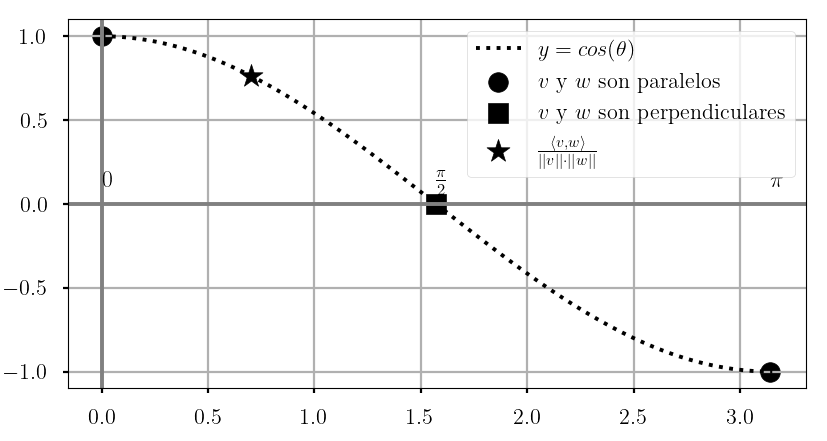
\includegraphics[scale=0.5]{coseno} 
\end{figure}	


Con esta definición de ángulo entre vectores, podemos 
trasladar la noción geométrica de ortogonalidad (i.e. de formar
un ángulo recto) al contexto de espacios con producto punto.
\begin{defi}
\label{def: ortogonalidad}
Sea $V$ un $F-$espacio vectorial con producto punto.
Dos elementos $v$ y $w$ del espacio se dirán
\textbf{ortogonales} si su producto punto es cero.
\end{defi}

Terminamos esta sección con una sencilla observación, que es 
consecuencia de la linealidad del producto punto y de la norma.

\begin{obs}
\label{obs: angulo se preserva por mult. esc.}
\textbf{(El ángulo entre dos vectores no se ve afectado
por multiplicación por un mismo escalar)}
Sean $V$ un espacio de Hilbert, $u, v \in V$ no cero.
Si $a \in F$ es un escalar no cero, entonces
$\measuredangle (v, w) = \measuredangle (a \cdot v, a \cdot w)$
\end{obs}

\subsection{Definición de ángulo entre un punto y un subespacio cerrado de un espacio euclideo}
\label{sec: def del angulo entre un punto y un subespacio cerrado}

Ya vimos en \ref{angulo entre elementos de un espacio con producto punto}
cómo definir el ángulo entre dos elementos de un espacio
de Hilbert $V$.

Si además $W$ es un subespacio cerrado de $V$
(cosa que siempre ocurre en caso que
$V$ sea finito dimensional, c.f. teorema 2.4-3 de \cite{Kreyszig}), entonces también
es posible definir el ángulo entre un punto $x \in V$
del espacio y $W$.

\begin{defi} \label{def: angulo punto subespacio}
Sea $(V, \langle \cdot , \cdot \rangle)$ un espacio con 
producto punto. Sean $W \leq V$ un subespacio cerrado de $V$
y $x \in V$. Definimos el \textbf{ángulo entre $x$ y $W$}
como el ángulo que forma 
$x$ con su proyección a $W$, es decir,
\[
\measuredangle (x, W):= \measuredangle(x, \Pi_{W}(x)).
\]
\end{defi}

Una definición alternativa del ángulo entre un punto y un subespacio,
así como una caracterización sencilla del coseno de este,
se dan a continuación.

\begin{prop}
\label{prop: algunos hechos sobre el angulo entre un vector y un subespacio}
Si $V$, $W$ y $x$ son como en la definición 
\ref{def: angulo punto subespacio}, entonces

\begin{itemize}
\item 
$\measuredangle (x, W) = min \{ \measuredangle(x,w) \hspace{0.1cm} :
 \hspace{0.1cm} w \in W \}$, y

\item 
\begin{equation}
\label{eq: coseno a subespacio}
cos \left( \measuredangle (x, W) \right) = \frac{|| \Pi_{W}(x) ||}{||x||}.
\end{equation}
\end{itemize}


\end{prop}
\noindent
\textbf{Demostración.}
\begin{itemize}
\item  Sea $w$ un elemento cualquiera de $W$.
Puesto que el ángulo entre dos vectores es
preservado bajo multiplicación por escalares
(c.f. observación
\ref{obs: angulo se preserva por mult. esc.}), sin pérdida de generalidad
podemos suponer que 
\begin{equation}
\label{eq1: 9Feb}
||w||= || \Pi_{W}(x)||.
\end{equation}

De la definición del vector $\Pi_{W}(x)$ se sigue que
\[
|| x -\Pi_{W}(x) ||^{2} \leq  || x - w||^{2};
\]
expresando ambos lados de la desigualdad como un producto
punto (c.f. \eqref{eq: norma via producto punto}) y aplicando la
bilinealidad del producto punto, llegamos a que
\[
\langle x , x \rangle -2 \langle x, \Pi_{W}(x) \rangle +
\langle \Pi_{W}(x) , \Pi_{W}(x) \rangle \leq 
\langle x , x \rangle  -2 \langle x , w \rangle 
+ \langle w , w \rangle ;
\]
usando \eqref{eq1: 9Feb}, podemos simplificar esta
última desigualdad para llegar a 
\[
\langle x, w \rangle \leq \langle x, \Pi_{W}(x) \rangle,
\]
de donde se sigue, usando nuevamente \eqref{eq1: 9Feb},
que 
\[
cos \left( \measuredangle (x,w) \right) =
\frac{\langle x , w \rangle}{||x||\cdot ||w||} \leq
\frac{\langle x ,  \Pi_{W}(x)  \rangle}{||x||\cdot ||\Pi_{W}(x) ||} =
cos \left( \measuredangle \left(x, \Pi_{W}(x) \right) \right);
\]
del que la función coseno sea decreciente en el intervalo
$[0, \pi]$ se concluye de esta última desigualdad que
$ \measuredangle \left(x, \Pi_{W}(x) \right) \leq 
\measuredangle (x,w)$.

\item Según el corolario 
\ref{cor: x como suma de proyecciones}, 
$x$ puede expresarse como la suma entre su proyección
a $W$ y su proyección a $W^{\perp}$, luego,
según la definición \ref{def: angulo punto subespacio}
y la linealidad del producto punto, concluimos que

\begin{align*}
cos \left( \measuredangle (x, W) \right) = &
cos \left( \measuredangle (x, \Pi_{W}(x)) \right)  \\
= & 
\frac{\langle x , \Pi_{W}(x) \rangle}{||x|| \cdot || \Pi_{W}(x)||}  \\
= & 
\frac{\langle \Pi_{W}(x)+\Pi_{W\perp}(x) , \Pi_{W}(x) \rangle}{||x|| \cdot || \Pi_{W}(x)||}\\
= & \frac{\langle \Pi_{W}(x) , \Pi_{W}(x) \rangle}{||x|| \cdot || \Pi_{W}(x)||}\\
= & \frac{|| \Pi_{W}(x) ||^{2}}{||x|| \cdot || \Pi_{W}(x)||}\\
= & \frac{|| \Pi_{W}(x) ||}{||x||}.
\end{align*}
\end{itemize}

\QEDB
\vspace{0.2cm}

\begin{nota}
Observe que, según el segundo punto de la proposición 
\ref{prop: algunos hechos sobre el angulo entre un vector y un subespacio}, 
el coseno entre un vector $x$ y un subespacio cerrado $W$ es
siempre no negativo; esto nos permite acotar el rango en el que
se encuentra el ángulo (que, por definición, es $[0, \pi]$)
y afirmar que $\measuredangle(x, W) \in [0, \frac{\pi}{2}]$.
\end{nota}

\subsection{Similitud coseno}
\label{cosine similarity}

Sea $V$ un espacio de Hilbert.
Sean $W \subseteq V$ un subespacio cerrado de $V$ y 
$x$ un elemento cualquiera de $V$. Hay dos formas ``naturales''
de intentar medir la cercanía de $x$ a $W$:
\begin{itemize}
\item[a)] \textbf{Usando la distancia euclídea
de $x$ a $W$}, es decir, tomando la norma del vector
$x - \Pi_{W}(x)$ como una medida
de qué tanto pertenece $x$ a $W$.
\item[b)] \textbf{Usando el ángulo que $x$ forma con $W$}: como ya
vimos en la sección 
\ref{sec: def del angulo entre un punto y un subespacio cerrado}, el ángulo 
$\measuredangle (x, W) \in [0, \frac{\pi}{2}]$
entre $x$ y $W$
está definido como el ángulo entre $x$ y su proyección
$\Pi_{W}(x)$ a $W$, luego, 
	\begin{itemize}
		\item entre más cercano a cero sea $\measuredangle (x, W)$,
		$x$ se aleja más del plano $W$, pues es casi perpendicular 
		al elemento de $W$ más cercano a $x$, y
		
		\item entre más cercano a uno sea $\measuredangle (x, W)$,
		más se acerca $x$ a ser paralelo a su representante en $W$,
		luego, más se acerca $x$ a pertenecer a $W$.
	\end{itemize}
\end{itemize}

\begin{figure}[H]
	\sidecaption{
	Esquema de dos formas en las que uno puede intentar medir
	la proximidad de un elemento $x \in V$ al subespacio cerrado $W$.
	\label{fig: dos formas de medir distancia a plano}
	}
	\centering
	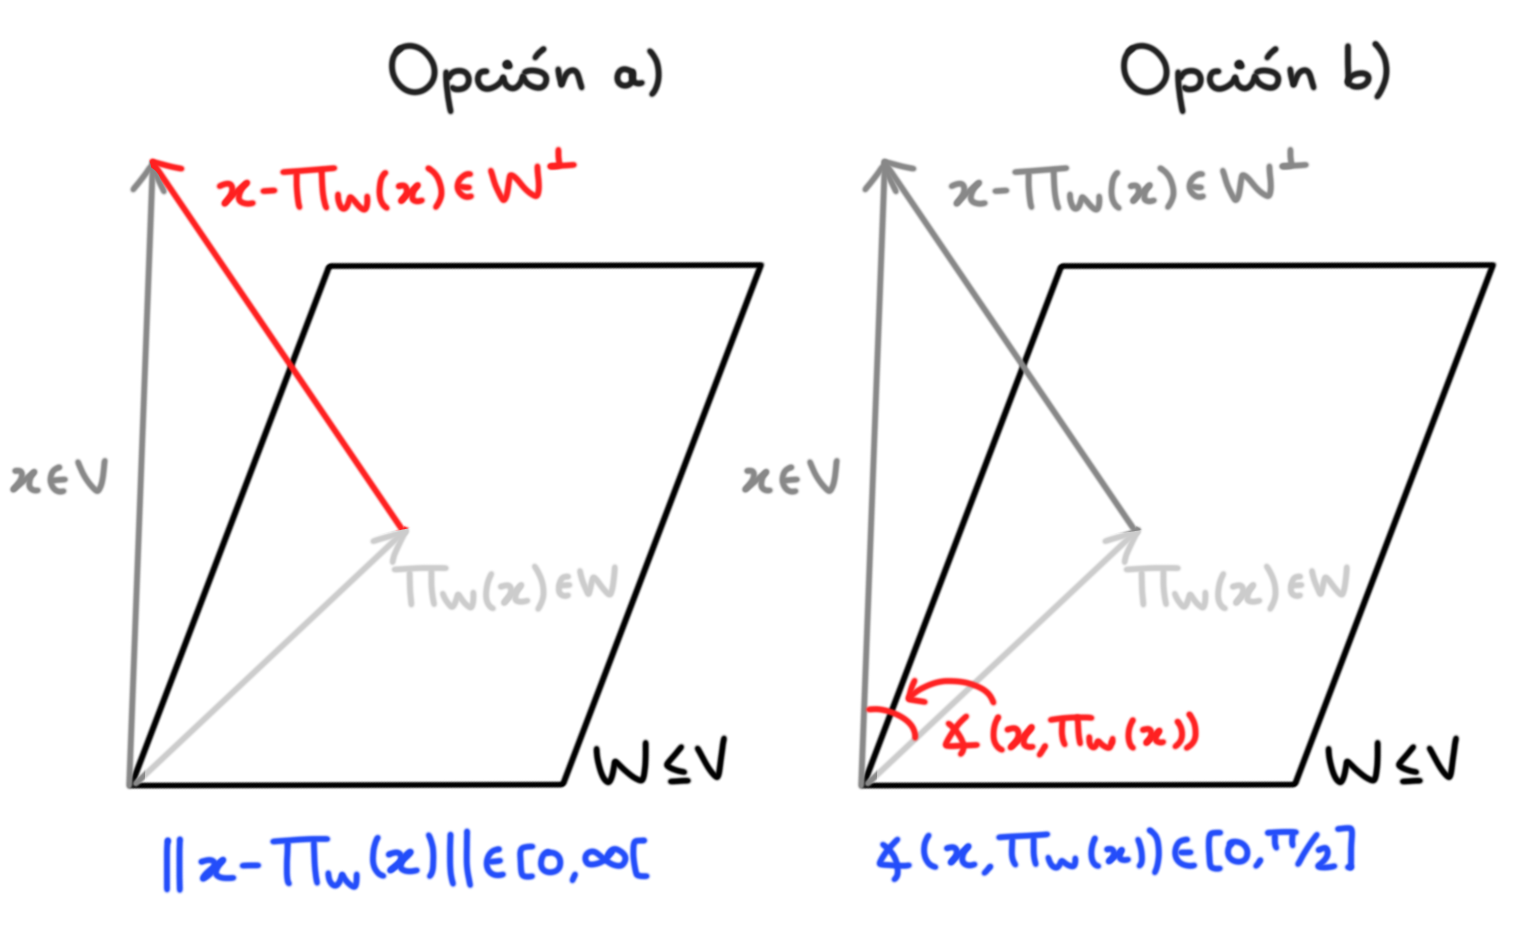
\includegraphics[scale=0.9]{18Sept_1} 
\end{figure}	

Este segundo
enfoque es conocido como ``\textbf{cosine similarity}'' en
inglés (c.f. \cite{cosineSim}). Una ventaja (que será decisiva
para nosotros) del segundo método sobre el primero se
expone en el siguiente resultado.


\begin{prop}
\label{prop: angulo se conserva bajo mult. esc.}
Sean $V$ un espacio euclideo, $W \subseteq V$ cerrado, $x \in V$,
$a \in \IR - \{ 0 \}$. Si $|a| \neq 1$, la distancia euclídea 
de $a \cdot x$ a $W$ es distinta
a la de $x$ a $W$, mientras que los 
ángulos que forman $a \cdot x$ y $x$
con $W$ coinciden.
\end{prop}
\noindent
\textbf{Demostración.}
En efecto, 

\[
|| a \cdot x - \Pi_{W}(a \cdot x) || = |a| \cdot || x - \Pi_{W}(x) ||
\neq || x - \Pi_{W}(x) ||, 
\]
mientras que

\begin{align*}
\measuredangle (a \cdot x, W):=& \measuredangle(a \cdot x, \Pi_{W}(a \cdot x)) \\
= & \frac{\langle a \cdot x , \Pi_{W}(a \cdot x) \rangle}{|| a \cdot x || \cdot 
|| \Pi_{W}(a \cdot x)  ||} \\
= & \frac{a^{2}  \langle   x , \Pi_{W}(x) \rangle}{a^{2} ||  x || \cdot 
|| \Pi_{W}( x)  ||}  \\
= & \measuredangle (x, W).
\end{align*}


\QEDB
\vspace{0.2cm}

Así el criterio $b)$ no se ve afectado por multiplicación escalar,
mientras que el $a)$ sí.
 


